%! suppress = Unicode
\documentclass[12pt, a4paper]{article}
\usepackage[utf8]{inputenc}
\usepackage{amsmath}
\usepackage{amsthm}
\usepackage{mathtools}
\usepackage[russian]{babel}
\usepackage{eucal}
\usepackage{blindtext}
\usepackage{fullpage}
\usepackage{tikz-cd}
\usepackage{centernot}
\usepackage{polynom}
\usepackage{tensor}
\usepackage{mleftright}
\usepackage{amssymb}
\usepackage[left=3cm, top=2cm, right=2cm, bottom=20mm, nohead, nofoot]{geometry}
\newcommand{\tle}{\trianglelefteq}
\newcommand{\tl}{\triangleleft}
\newcommand{\R}{\mathbb{R}}
\newcommand{\F}{\mathbb{F}}
\newcommand{\Z}{\mathbb{Z}}
\newcommand{\Q}{\mathbb{Q}}
\newcommand{\N}{\mathbb{N}}
\renewcommand{\C}{\mathbb{C}}


\title{\textbf{Отчет по лабораторной работе \textnumero{1}}}

\medskip

\author{Гусаров Евгений, Шиманская Маргарита
\\М3237}
\usepackage{natbib}
\usepackage{graphicx}
\usepackage{textcomp}
\usepackage{tikz}
\usepackage[T1]{fontenc}

\begin{document}
    \maketitle
    \newpage


    \section{Постановка задачи}\label{sec:постановка-задачи}
    \Large\textit{Вариант \textnumero{3}}
    \\
    \\
    \Large\textit{$f(x) = x \cdot \sin(x) + 2 \cdot \cos(x)$}
    \\
    \\
    \Large{Найти минимум данной функции на отрезке $[-6; -4]$, реализовав алгоритмы одномерной минимизации функции:}
    \begin{itemize}
        \item {метод дихтомии}
        \item {метод золотого сечения}
        \item {метод Фиббоначи}
        \item {метод парабол}
        \item {комбинированный метод Брента}
    \end{itemize}

    \Large{Сравнить результат работы с аналитическим решением данной задачи, сделать выводы.}


    \newpage


    \section{Аналитическое решение}\label{sec:аналитическое-решение}
    \begin{figure}[h]
        \center{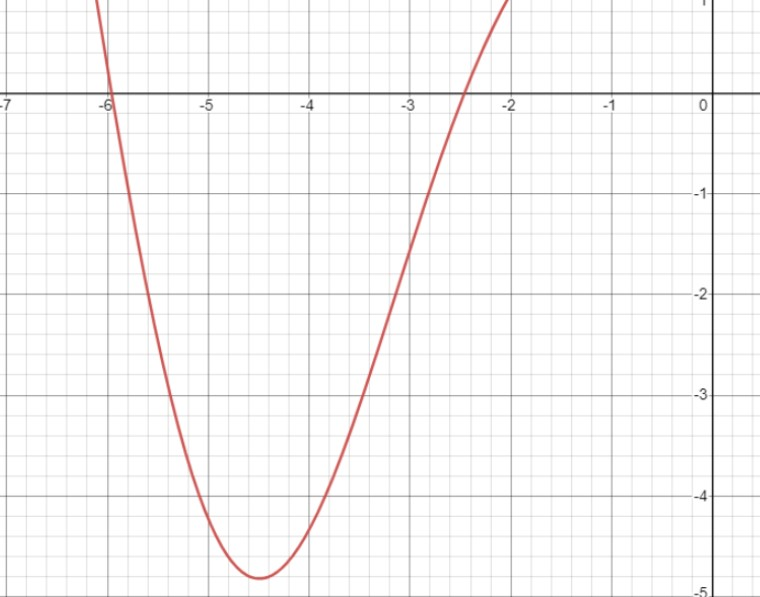
\includegraphics[scale=0.5]{graphic}}
        \caption{График функции}
        \label{fig:image}
    \end{figure}
    \\
    \Large{$f(x) = x \cdot \sin(x) + 2 \cdot \cos(x)$}
    \\
    \Large{$f'(x) = x \cdot \cos(x)  + \sin(x) - 2 \cdot \sin(x)$}
    \\
    \Large{$f'(x) = 0$}
    \qquad
    \Large{$<=>$}
    \qquad
    \Large{$x \cdot \cos(x) - \sin(x) = 0$}
    \\
    \Large{$x = \tan(x)$}
    \\
    \Large{На данном отрезке один корень: $x_1 \approx -4.4934$}
    \\
    \Large{$f(x_1) \approx -4.8206$}
    \\
    \Large{Функция достигает минимума в этой точке. потому что на интервале $(x_1 - \epsilon ; x_1)$ функция убывает(производная < 0), а на $(x_1; x_1 + \epsilon )$ возрастает(производная > 0)}
    \newpage


    \section{Результаты исследований методов}\label{sec:результаты-исследований-методов}
    \subsection{Метод дихотомии}\label{subsec:метод-дихотомии}
\begin{center}
    \begin{tabular}{ | l | l | l | l | l | l |}
        \hline
        \textnumero{} & left        & right       & length     & $x$         & $f(x)$      \\ \hline
        1             & -6,00000000 & -4,00000000 & 2,00000000 & -5,00000050 & -4,22729581 \\
        2             & -6,00000000 & -4,00000000 & 2,00000000 & -4,99999950 & -4,22729819 \\
        3             & -5,00000050 & -4,00000000 & 1,00000050 & -4,50000075 & -4,82047711 \\
        4             & -5,00000050 & -4,00000000 & 1,00000050 & -4,49999975 & -4,82047714 \\
        5             & -4,50000075 & -4,00000000 & 0,50000075 & -4,25000087 & -4,69588063 \\
        6             & -4,50000075 & -4,00000000 & 0,50000075 & -4,24999987 & -4,69587963 \\
        7             & -4,50000075 & -4,24999987 & 0,25000087 & -4,37500081 & -4,79039632 \\
        8             & -4,50000075 & -4,24999987 & 0,25000087 & -4,37499981 & -4,79039581 \\
        9             & -4,50000075 & -4,37499981 & 0,12500094 & -4,43750078 & -4,81377593 \\
        10            & -4,50000075 & -4,37499981 & 0,12500094 & -4,43749978 & -4,81377569 \\
        11            & -4,50000075 & -4,43749978 & 0,06250097 & -4,46875077 & -4,81924393 \\
        12            & -4,50000075 & -4,43749978 & 0,06250097 & -4,46874977 & -4,81924382 \\
        13            & -4,50000075 & -4,46874977 & 0,03125098 & -4,48437576 & -4,82039375 \\
        14            & -4,50000075 & -4,46874977 & 0,03125098 & -4,48437476 & -4,82039371 \\
        15            & -4,50000075 & -4,48437476 & 0,01562599 & -4,49218825 & -4,82056921 \\
        16            & -4,50000075 & -4,48437476 & 0,01562599 & -4,49218725 & -4,82056920 \\
        17            & -4,50000075 & -4,49218725 & 0,00781350 & -4,49609450 & -4,82055666 \\
        18            & -4,50000075 & -4,49218725 & 0,00781350 & -4,49609350 & -4,82055667 \\
        19            & -4,49609450 & -4,49218725 & 0,00390725 & -4,49414138 & -4,82057130 \\
        20            & -4,49609450 & -4,49218725 & 0,00390725 & -4,49414038 & -4,82057131 \\
        21            & -4,49414138 & -4,49218725 & 0,00195412 & -4,49316482 & -4,82057235 \\
        22            & -4,49414138 & -4,49218725 & 0,00195412 & -4,49316382 & -4,82057234 \\
        23            & -4,49414138 & -4,49316382 & 0,00097756 & -4,49365310 & -4,82057235 \\
        24            & -4,49414138 & -4,49316382 & 0,00097756 & -4,49365210 & -4,82057235 \\
        25            & -4,49365310 & -4,49316382 & 0,00048928 & -4,49340896 & -4,82057248 \\
        26            & -4,49365310 & -4,49316382 & 0,00048928 & -4,49340796 & -4,82057248 \\ \hline
    \end{tabular}
    \begin{tabular}{ | l | l | l | l | l | l |}
        \hline
        \textnumero{} & left        & right       & length     & $x$         & $f(x)$      \\ \hline
        27            & -4,49365310 & -4,49340796 & 0,00024514 & -4,49353103 & -4,82057244 \\
        28            & -4,49365310 & -4,49340796 & 0,00024514 & -4,49353003 & -4,82057245 \\
        29            & -4,49353103 & -4,49340796 & 0,00012307 & -4,49346999 & -4,82057247 \\
        30            & -4,49353103 & -4,49340796 & 0,00012307 & -4,49346899 & -4,82057247 \\
        31            & -4,49346999 & -4,49340796 & 0,00006204 & -4,49343947 & -4,82057247 \\
        32            & -4,49346999 & -4,49340796 & 0,00006204 & -4,49343847 & -4,82057248 \\
        33            & -4,49343947 & -4,49340796 & 0,00003152 & -4,49342422 & -4,82057248 \\
        34            & -4,49343947 & -4,49340796 & 0,00003152 & -4,49342322 & -4,82057248 \\ \hline
    \end{tabular}
\end{center}

\subsubsection{Вывод}
{Из графика \textnumero{2} видно, что количество вычислений функции для метода дихотомии линейно зависит от $\log\epsilon$. \\

Плюсы данного метода: \\
1. Простота в написании. \\
2. При уменьшении $\Delta$ повышается скорость сходимости. \\

Минусы данного метода: \\
1. На каждой итерации вычисляется значение функции в двух точках, что негативно отражается на скорости. \\
2. При чрезмерно малом $\Delta$ сравнение точек становится затруднительным.}
\newpage

\subsection{Метод золотого сечения}\label{subsec:метод-золотого-сечения}
\begin{center}
    \begin{tabular}{ | l | l | l | l | l | l |}
        \hline
        \textnumero{} & left        & right       & length     & $x$         & $f(x)$      \\ \hline
        1             & -6,00000000 & -4,00000000 & 2,00000000 & -5,23606798 & -3,53421890 \\
        2             & -6,00000000 & -4,00000000 & 2,00000000 & -4,76393202 & -4,65456484 \\
        3             & -5,23606798 & -4,00000000 & 1,23606798 & -4,47213595 & -4,81958315 \\
        4             & -4,76393202 & -4,00000000 & 0,76393202 & -4,29179607 & -4,73435675 \\
        5             & -4,76393202 & -4,29179607 & 0,47213595 & -4,58359214 & -4,80250900 \\
        6             & -4,58359214 & -4,29179607 & 0,29179607 & -4,40325225 & -4,80299576 \\
        7             & -4,58359214 & -4,40325225 & 0,18033989 & -4,51470843 & -4,81957450 \\
        8             & -4,51470843 & -4,40325225 & 0,11145618 & -4,44582472 & -4,81564263 \\
        9             & -4,51470843 & -4,44582472 & 0,06888371 & -4,48839719 & -4,82051742 \\
        10            & -4,51470843 & -4,47213595 & 0,04257247 & -4,49844719 & -4,82051678 \\
        11            & -4,49844719 & -4,47213595 & 0,02631123 & -4,48218595 & -4,82029669 \\
        12            & -4,49844719 & -4,48218595 & 0,01626124 & -4,49223595 & -4,82056946 \\
        13            & -4,49844719 & -4,48839719 & 0,01005000 & -4,49460843 & -4,82056932 \\
        14            & -4,49460843 & -4,48839719 & 0,00621124 & -4,49076968 & -4,82055720 \\
        15            & -4,49460843 & -4,49076968 & 0,00383876 & -4,49314216 & -4,82057232 \\
        16            & -4,49460843 & -4,49223595 & 0,00237248 & -4,49370222 & -4,82057229 \\
        17            & -4,49370222 & -4,49223595 & 0,00146627 & -4,49279602 & -4,82057165 \\
        18            & -4,49370222 & -4,49279602 & 0,00090621 & -4,49335608 & -4,82057247 \\
        19            & -4,49370222 & -4,49314216 & 0,00056007 & -4,49348830 & -4,82057246 \\
        20            & -4,49348830 & -4,49314216 & 0,00034614 & -4,49327437 & -4,82057244 \\
        21            & -4,49348830 & -4,49327437 & 0,00021393 & -4,49340659 & -4,82057248 \\
        22            & -4,49348830 & -4,49335608 & 0,00013221 & -4,49343780 & -4,82057248 \\
        23            & -4,49343780 & -4,49335608 & 0,00008171 & -4,49338730 & -4,82057248 \\
        24            & -4,49343780 & -4,49338730 & 0,00005050 & -4,49341851 & -4,82057248 \\
        25            & -4,49341851 & -4,49338730 & 0,00003121 & -4,49339922 & -4,82057248 \\
        26            & -4,49341851 & -4,49339922 & 0,00001929 & -4,49341114 & -4,82057248 \\ \hline
    \end{tabular}
\end{center}

\subsubsection{Вывод}
{Из графика \textnumero{2} видно, что количество вычислений функции для метода золотого сечения линейно зависит от $\log\epsilon$. \\

Плюсы данного метода: \\
1. Требует меньшего числа вычислений функции, чем метод дихотомии, потому что на каждом промежутке вычисляется только одно новое значение $x$ и $f(x)$. \\
2. Не вычисляются значения в крайних точках. \\

Минусы данного метода: \\
1. Быстро накапливается погрешность из-за того, что константа $\phi=\frac{\sqrt{5}-1}{2}$ представляется в ЭВМ неточно. \\

Стоит отметить, что результат алгоритма с уменьшением количества итераций почти не меняется относительно $\varepsilon$.}
\newpage

\subsection{Метод Фибоначчи}\label{subsec:метод-фибоначчи}
\begin{center}
    \begin{tabular}{ | l | l | l | l | l | l |}
        \hline
        \textnumero{} & left        & right       & length     & $x$         & $f(x)$      \\ \hline
        1             & -6,00000000 & -4,00000000 & 2,00000000 & -5,23606798 & -3,53421890 \\
        2             & -6,00000000 & -4,00000000 & 2,00000000 & -4,76393202 & -4,65456484 \\
        3             & -5,23606798 & -4,00000000 & 1,23606798 & -4,47213596 & -4,81958315 \\
        4             & -4,76393202 & -4,00000000 & 0,76393202 & -4,29179607 & -4,73435675 \\
        5             & -4,76393202 & -4,29179607 & 0,47213596 & -4,58359213 & -4,80250900 \\
        6             & -4,58359213 & -4,29179607 & 0,29179607 & -4,40325225 & -4,80299576 \\
        7             & -4,58359213 & -4,40325225 & 0,18033989 & -4,51470843 & -4,81957450 \\
        8             & -4,51470843 & -4,40325225 & 0,11145618 & -4,44582472 & -4,81564263 \\
        9             & -4,51470843 & -4,44582472 & 0,06888371 & -4,48839719 & -4,82051742 \\
        10            & -4,51470843 & -4,47213596 & 0,04257247 & -4,49844719 & -4,82051678 \\
        11            & -4,49844719 & -4,47213596 & 0,02631124 & -4,48218595 & -4,82029669 \\
        12            & -4,49844719 & -4,48218595 & 0,01626124 & -4,49223595 & -4,82056946 \\
        13            & -4,49844719 & -4,48839719 & 0,01005000 & -4,49460843 & -4,82056932 \\
        14            & -4,49460843 & -4,48839719 & 0,00621124 & -4,49076967 & -4,82055720 \\
        15            & -4,49460843 & -4,49076967 & 0,00383876 & -4,49314215 & -4,82057232 \\
        16            & -4,49460843 & -4,49223595 & 0,00237248 & -4,49370223 & -4,82057229 \\
        17            & -4,49370223 & -4,49223595 & 0,00146628 & -4,49279603 & -4,82057165 \\
        18            & -4,49370223 & -4,49279603 & 0,00090620 & -4,49335611 & -4,82057247 \\
        19            & -4,49370223 & -4,49314215 & 0,00056008 & -4,49348827 & -4,82057246 \\
        20            & -4,49348827 & -4,49314215 & 0,00034612 & -4,49327430 & -4,82057244 \\
        21            & -4,49348827 & -4,49327430 & 0,00021396 & -4,49340646 & -4,82057248 \\
        22            & -4,49348827 & -4,49335611 & 0,00013215 & -4,49343792 & -4,82057248 \\
        23            & -4,49343792 & -4,49335611 & 0,00008181 & -4,49338758 & -4,82057248 \\
        24            & -4,49343792 & -4,49338758 & 0,00005034 & -4,49341904 & -4,82057248 \\
        25            & -4,49341904 & -4,49338758 & 0,00003147 & -4,49340017 & -4,82057248 \\
        26            & -4,49341904 & -4,49340017 & 0,00001888 & -4,49341275 & -4,82057248 \\
        27            & -4,49341275 & -4,49340017 & 0,00001259 & -4,49340646 & -4,82057248 \\ \hline
    \end{tabular}
\end{center}

\subsubsection{Вывод}
{Из графика \textnumero{2} видно, что количество вычислений функции для метода Фибоначчи линейно зависит от $\log\epsilon$. \\

Плюсы данного метода: \\
1. Не вычисляются значения в крайних точках. \\
2. Коэффициент сокращения интервала меняется от итерации к итерации. \\

В связи с этим метод Фибоначчи является более эффективным, чем метод золотого сечения\\
Стоит отметить, что количество итераций \textit{n} фиксировано, их нужно выбирать исходя из точности и начальной длины промежутка.}

\newpage

\subsection{Метод парабол}
\label{subsec:parabolasection}
\begin{center}
    \begin{tabular}{ | l | l | l | l | l | l |}
        \hline
        \textnumero{} & left        & right       & length     & $x$         & $f(x)$      \\ \hline
        1             & -6,00000000 & -4,00000000 & 2,00000000 & -6,00000000 & 0,24384758  \\
        2             & -6,00000000 & -4,00000000 & 2,00000000 & -5,00000000 & -4,22729700 \\
        3             & -6,00000000 & -4,00000000 & 2,00000000 & -4,00000000 & -4,33449722 \\
        4             & -6,00000000 & -4,00000000 & 2,00000000 & -4,47543502 & -4,81986585 \\
        5             & -5,00000000 & -4,00000000 & 1,00000000 & -4,47507589 & -4,81983737 \\
        6             & -5,00000000 & -4,47507589 & 0,52492411 & -4,49247153 & -4,82057055 \\
        7             & -5,00000000 & -4,47543502 & 0,52456498 & -4,49291712 & -4,82057195 \\
        8             & -5,00000000 & -4,49247153 & 0,50752847 & -4,49337272 & -4,82057247 \\
        9             & -5,00000000 & -4,49291712 & 0,50708288 & -4,49339587 & -4,82057248 \\
        10            & -5,00000000 & -4,49337272 & 0,50662728 & -4,49340817 & -4,82057248 \\
        11            & -5,00000000 & -4,49339587 & 0,50660413 & -4,49340908 & -4,82057248 \\
        \hline
    \end{tabular}
\end{center}

\subsubsection{Вывод}
{Из графика \textnumero{2} видно, что количество вычислений функции для метода парабол линейно зависит от $\log\epsilon$. \\

Плюсы данного метода: \\
1. В общем случае метод парабол обладает суперлинейной скоростью сходимости. \\
2. Меньше итераций по сравнению с предыдущими методами. \\

Минусы данного метода: \\
1. Требует вычисления значений в крайних точках функции и нахождения промежуточной точки, удовлетворяющей неравенству на первой итерации. \\
2. Высокая скорость сходимости гарантируется только в малой окрестности точки минимума. \\}

\newpage

\subsection{Метод Брента}
\label{subsec:brentsection}
\begin{center}
    \begin{tabular}{ | l | l | l | l | l | l |}
        \hline
        \textnumero{} & left        & right       & length     & $x$         & $f(x)$      \\ \hline
        1             & -6,00000000 & -4,00000000 & 2,00000000 & -5,23606798 & -3,53421890 \\
        2             & -6,00000000 & -4,00000000 & 2,00000000 & -4,76393202 & -4,65456484 \\
        3             & -5,23606798 & -4,00000000 & 1,23606798 & -4,47213595 & -4,81958315 \\
        4             & -4,76393202 & -4,00000000 & 0,76393202 & -4,49851910 & -4,82051518 \\
        5             & -4,76393202 & -4,47213595 & 0,29179607 & -4,49312987 & -4,82057231 \\
        6             & -4,49851910 & -4,47213595 & 0,02638314 & -4,49340165 & -4,82057248 \\
        7             & -4,49851910 & -4,49312987 & 0,00538922 & -4,49340935 & -4,82057248 \\
        8             & -4,49851910 & -4,49340165 & 0,00511745 & -4,49341273 & -4,82057248 \\
        9             & -4,49341273 & -4,49340165 & 0,00001108 & -4,49340597 & -4,82057248 \\
        \hline
    \end{tabular}
\end{center}

\subsubsection{Вывод}
{Из графика \textnumero{2} видно, что количество вычислений функции для комбинированного метода Брента линейно зависит от $\log\epsilon$. \\

Плюсы данного метода: \\
1. Эффективно комбинирует метод золотого сечения и метод парабол. \\
2. Меньше всего вычислений функции. (Возможно, нам повезло с функцией) \\

Минусы данного метода: \\
1. Сложность реализации по сравнению с остальными методами.}


\begin{figure}[h]
    \center{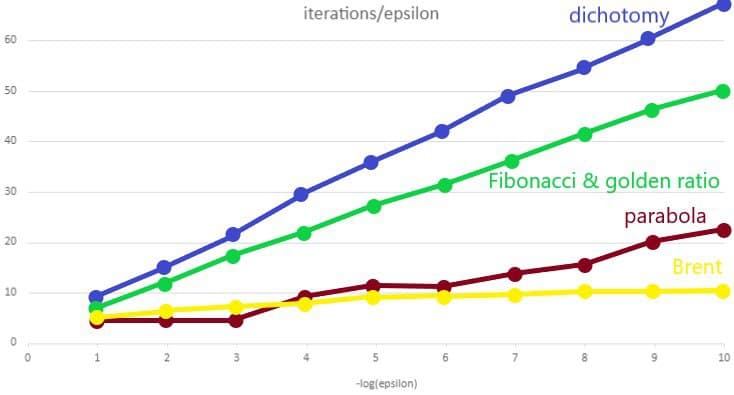
\includegraphics[scale=0.5]{iterations-epsilon}}
    \caption{Зависимость количества итераций от $\log\epsilon$}
    \label{fig:image}
\end{figure}

\newpage


    \section{Тестирование алгоритмов на многомодальной функции}\label{sec:тестирование-алгоритмов-на-многомодальной-функции}
    {Приведённые алгоритмы работают при поиске минимума унимодальной функции.
    Оценим результаты их работы на многомодальной функции, например, вида $f(x)=-x^{\cos(x)}\exp(\sin(x)$) на отрезке. \(x = \left[0, 20\right]\)}

    \begin{figure}[h]
        \center{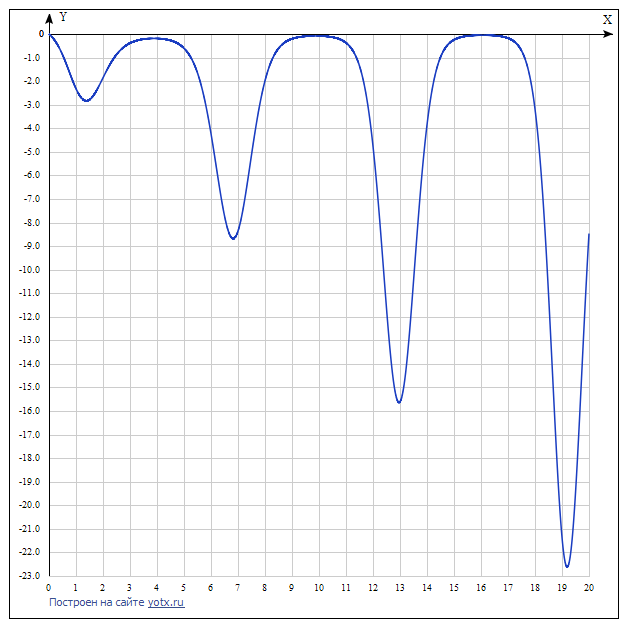
\includegraphics[scale=0.5]{manyModalsGraphic}}
        \caption{График функции}
        \label{fig:image}
    \end{figure}
    \noindent
    {Для теста был выбран $\varepsilon=0.00000001$.
    Аналитическим решением получили точку минимума: $x \approx 19.1916598$.}

    {Ниже приведены результаты работы алгоритмов на данной функции.}

    \begin{table}[h!]
        \begin{center}
            \begin{tabular}{|c c c|}
                \hline

                {Метод}         & Число итераций & результат          \\
                \hline
                Дихотомия       & 60             & 12.964333547131023 \\
                Золотое сечение & 46             & 12.964333604846322 \\
                Фибоначчи       & 46             & 12.964333592016619 \\
                Метод Парабол   & 17             & 6.82151365682379   \\
                Метод Брента    & 14             & 12.964333590155599 \\
                \hline
            \end{tabular}
        \end{center}\label{tab:table}
    \end{table}

    \noindent
    {Как видно все методы нашли точки локального минимума $x \approx 6.82151365682379$ и $x \approx 12.964333590155599$.
    Ни один метод не смог найти точку глобального минимума.
    Эти результаты показывают, что данные методы не могут гарантировать корректный результат на многомодальных функциях.}


    \section{Результаты исследования}\label{sec:результаты-исследования}
    {В ходе работы нами были реализованы и протестированны пять алгоритмов поиска минимума унимодальной функции.
    Метод Брента оказался наиболее устойчивым.
    Также методу Брента потребовалось меньше всего итераций и вычислений функции для нахождения ответа.

    Кроме того мы протестировали алгоритмы на многомодальных функциях.
    Все методы выдали точки локальных минимумов, а не глобального.
    Исходя из этого можно понять, что лучше не стоит применять данные алгоритмы для поиска минимума в многомодальных функциях.}

\end{document}